\documentclass{standalone}
\usepackage{tikz}
\usetikzlibrary{patterns, positioning}

\begin{document}
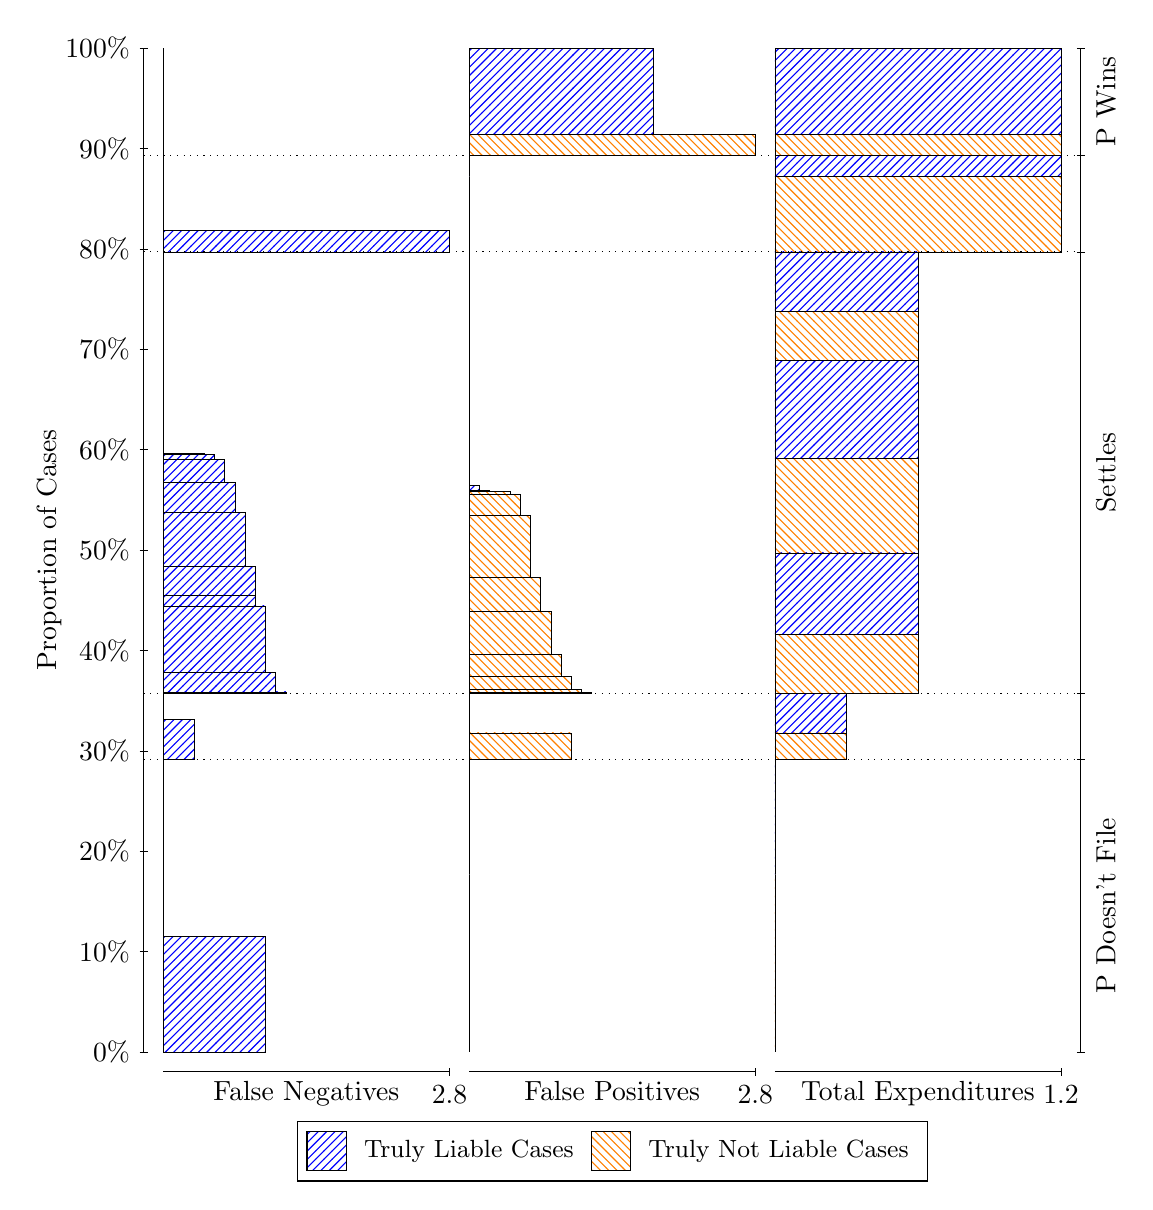
\begin{tikzpicture}
\draw[black, very thin] (1.5,1.75) -- (1.5,14.5);
\node[rotate=90, anchor=center] at (0.3, 8.125) {Proportion of Cases};
\draw[black, very thin] (1.45,1.75) -- (1.55,1.75);
\node[anchor=east] at (1.45, 1.75) {0\%};
\draw[black, very thin] (1.45,3.025) -- (1.55,3.025);
\node[anchor=east] at (1.45, 3.025) {10\%};
\draw[black, very thin] (1.45,4.3) -- (1.55,4.3);
\node[anchor=east] at (1.45, 4.3) {20\%};
\draw[black, very thin] (1.45,5.575) -- (1.55,5.575);
\node[anchor=east] at (1.45, 5.575) {30\%};
\draw[black, very thin] (1.45,6.85) -- (1.55,6.85);
\node[anchor=east] at (1.45, 6.85) {40\%};
\draw[black, very thin] (1.45,8.125) -- (1.55,8.125);
\node[anchor=east] at (1.45, 8.125) {50\%};
\draw[black, very thin] (1.45,9.4) -- (1.55,9.4);
\node[anchor=east] at (1.45, 9.4) {60\%};
\draw[black, very thin] (1.45,10.675) -- (1.55,10.675);
\node[anchor=east] at (1.45, 10.675) {70\%};
\draw[black, very thin] (1.45,11.95) -- (1.55,11.95);
\node[anchor=east] at (1.45, 11.95) {80\%};
\draw[black, very thin] (1.45,13.225) -- (1.55,13.225);
\node[anchor=east] at (1.45, 13.225) {90\%};
\draw[black, very thin] (1.45,14.5) -- (1.55,14.5);
\node[anchor=east] at (1.45, 14.5) {100\%};

\draw[black, very thin] (13.4,1.75) -- (13.4,14.5);
\draw[black, very thin] (13.35,1.75) -- (13.45,1.75);
\node[anchor=west] at (13.35, 1.75) {};
\draw[black, very thin] (13.35,5.468) -- (13.45,5.468);
\node[anchor=west] at (13.35, 5.468) {};
\draw[black, very thin] (13.35,6.3077) -- (13.45,6.3077);
\node[anchor=west] at (13.35, 6.3077) {};
\draw[black, very thin] (13.35,11.912) -- (13.45,11.912);
\node[anchor=west] at (13.35, 11.912) {};
\draw[black, very thin] (13.35,13.139) -- (13.45,13.139);
\node[anchor=west] at (13.35, 13.139) {};
\draw[black, very thin] (13.35,14.5) -- (13.45,14.5);
\node[anchor=west] at (13.35, 14.5) {};

\draw[black, very thin, pattern color=blue, pattern=north east lines] (1.75,1.75) rectangle (3.0476,3.2143);
\draw[black, very thin, pattern color=orange, pattern=north west lines] (1.75,3.2143) rectangle (1.75,5.468);
\draw[black, very thin, pattern color=blue, pattern=north east lines] (1.75,5.468) rectangle (2.1393,5.9738);
\draw[black, very thin, pattern color=orange, pattern=north west lines] (1.75,5.9738) rectangle (1.75,6.3077);
\draw[black, very thin, pattern color=blue, pattern=north east lines] (1.75,6.3077) rectangle (3.3071,6.3229);
\draw[black, very thin, pattern color=blue, pattern=north east lines] (1.75,6.3229) rectangle (3.1774,6.5686);
\draw[black, very thin, pattern color=blue, pattern=north east lines] (1.75,6.5686) rectangle (3.0476,7.4156);
\draw[black, very thin, pattern color=blue, pattern=north east lines] (1.75,7.4156) rectangle (2.9179,7.5524);
\draw[black, very thin, pattern color=blue, pattern=north east lines] (1.75,7.5524) rectangle (2.9179,7.9125);
\draw[black, very thin, pattern color=blue, pattern=north east lines] (1.75,7.9125) rectangle (2.7881,8.6016);
\draw[black, very thin, pattern color=blue, pattern=north east lines] (1.75,8.6016) rectangle (2.6583,8.9872);
\draw[black, very thin, pattern color=blue, pattern=north east lines] (1.75,8.9872) rectangle (2.5286,9.2786);
\draw[black, very thin, pattern color=blue, pattern=north east lines] (1.75,9.2786) rectangle (2.3988,9.3365);
\draw[black, very thin, pattern color=blue, pattern=north east lines] (1.75,9.3365) rectangle (2.269,9.3524);
\draw[black, very thin, pattern color=orange, pattern=north west lines] (1.75,9.3524) rectangle (1.75,11.912);
\draw[black, very thin, pattern color=blue, pattern=north east lines] (1.75,11.912) rectangle (5.3833,12.18);
\draw[black, very thin, pattern color=orange, pattern=north west lines] (1.75,12.18) rectangle (1.75,13.139);
\draw[black, very thin, pattern color=orange, pattern=north west lines] (1.75,13.139) rectangle (1.75,13.408);
\draw[black, very thin, pattern color=blue, pattern=north east lines] (1.75,13.408) rectangle (1.75,14.5);
\draw[black, very thin, pattern color=orange, pattern=north west lines] (5.6333,1.75) rectangle (5.6333,4.0036);
\draw[black, very thin, pattern color=blue, pattern=north east lines] (5.6333,4.0036) rectangle (5.6333,5.468);
\draw[black, very thin, pattern color=orange, pattern=north west lines] (5.6333,5.468) rectangle (6.931,5.8019);
\draw[black, very thin, pattern color=blue, pattern=north east lines] (5.6333,5.8019) rectangle (5.6333,6.3077);
\draw[black, very thin, pattern color=orange, pattern=north west lines] (5.6333,6.3077) rectangle (7.1905,6.3206);
\draw[black, very thin, pattern color=orange, pattern=north west lines] (5.6333,6.3206) rectangle (7.0607,6.3556);
\draw[black, very thin, pattern color=orange, pattern=north west lines] (5.6333,6.3556) rectangle (6.931,6.5231);
\draw[black, very thin, pattern color=orange, pattern=north west lines] (5.6333,6.5231) rectangle (6.8012,6.804);
\draw[black, very thin, pattern color=orange, pattern=north west lines] (5.6333,6.804) rectangle (6.6714,7.344);
\draw[black, very thin, pattern color=orange, pattern=north west lines] (5.6333,7.344) rectangle (6.5417,7.7811);
\draw[black, very thin, pattern color=orange, pattern=north west lines] (5.6333,7.7811) rectangle (6.4119,8.5656);
\draw[black, very thin, pattern color=orange, pattern=north west lines] (5.6333,8.5656) rectangle (6.2821,8.8332);
\draw[black, very thin, pattern color=orange, pattern=north west lines] (5.6333,8.8332) rectangle (6.1524,8.8675);
\draw[black, very thin, pattern color=blue, pattern=north east lines] (5.6333,8.8675) rectangle (5.8929,8.8834);
\draw[black, very thin, pattern color=blue, pattern=north east lines] (5.6333,8.8834) rectangle (5.7631,8.9412);
\draw[black, very thin, pattern color=blue, pattern=north east lines] (5.6333,8.9412) rectangle (5.6333,11.912);
\draw[black, very thin, pattern color=orange, pattern=north west lines] (5.6333,11.912) rectangle (5.6333,12.871);
\draw[black, very thin, pattern color=blue, pattern=north east lines] (5.6333,12.871) rectangle (5.6333,13.139);
\draw[black, very thin, pattern color=orange, pattern=north west lines] (5.6333,13.139) rectangle (9.2667,13.408);
\draw[black, very thin, pattern color=blue, pattern=north east lines] (5.6333,13.408) rectangle (7.969,14.5);
\draw[black, very thin, pattern color=orange, pattern=north west lines] (9.5167,1.75) rectangle (9.5167,4.0036);
\draw[black, very thin, pattern color=blue, pattern=north east lines] (9.5167,4.0036) rectangle (9.5167,5.468);
\draw[black, very thin, pattern color=orange, pattern=north west lines] (9.5167,5.468) rectangle (10.425,5.8019);
\draw[black, very thin, pattern color=blue, pattern=north east lines] (9.5167,5.8019) rectangle (10.425,6.3077);
\draw[black, very thin, pattern color=orange, pattern=north west lines] (9.5167,6.3077) rectangle (11.333,7.0502);
\draw[black, very thin, pattern color=blue, pattern=north east lines] (9.5167,7.0502) rectangle (11.333,8.0886);
\draw[black, very thin, pattern color=orange, pattern=north west lines] (9.5167,8.0886) rectangle (11.333,9.2848);
\draw[black, very thin, pattern color=blue, pattern=north east lines] (9.5167,9.2848) rectangle (11.333,10.53);
\draw[black, very thin, pattern color=orange, pattern=north west lines] (9.5167,10.53) rectangle (11.333,11.151);
\draw[black, very thin, pattern color=blue, pattern=north east lines] (9.5167,11.151) rectangle (11.333,11.912);
\draw[black, very thin, pattern color=orange, pattern=north west lines] (9.5167,11.912) rectangle (13.15,12.871);
\draw[black, very thin, pattern color=blue, pattern=north east lines] (9.5167,12.871) rectangle (13.15,13.139);
\draw[black, very thin, pattern color=orange, pattern=north west lines] (9.5167,13.139) rectangle (13.15,13.408);
\draw[black, very thin, pattern color=blue, pattern=north east lines] (9.5167,13.408) rectangle (13.15,14.5);
\draw[black, dotted] (1.5,5.468) -- (13.4,5.468);
\draw[black, dotted] (1.5,6.3077) -- (13.4,6.3077);
\draw[black, dotted] (1.5,11.912) -- (13.4,11.912);
\draw[black, dotted] (1.5,13.139) -- (13.4,13.139);
\draw[black, very thin] (1.75,1.5) -- (5.3833,1.5);
\node[anchor=north] at (3.5667, 1.5) {False Negatives};
\draw[black, very thin] (5.3833,1.45) -- (5.3833,1.55);
\node[anchor=north] at (5.3833, 1.45) {2.8};

\draw[black, very thin] (5.6333,1.5) -- (9.2667,1.5);
\node[anchor=north] at (7.45, 1.5) {False Positives};
\draw[black, very thin] (9.2667,1.45) -- (9.2667,1.55);
\node[anchor=north] at (9.2667, 1.45) {2.8};

\draw[black, very thin] (9.5167,1.5) -- (13.15,1.5);
\node[anchor=north] at (11.333, 1.5) {Total Expenditures};
\draw[black, very thin] (13.15,1.45) -- (13.15,1.55);
\node[anchor=north] at (13.15, 1.45) {1.2};

\node[black, centered, rotate=90] at (13.72, 3.609) {P Doesn't File};

\node[black, centered, rotate=90] at (13.72, 9.1099) {Settles};

\node[black, centered, rotate=90] at (13.72, 13.82) {P Wins};

\draw (7.449999999999999,1.5) node[draw=none] (baseCoordinate) {};
\begin{scope}[align=center]
        \matrix[scale=0.5, draw=black, below=0.5cm of baseCoordinate, nodes={draw}, column sep=0.1cm]{
            \node[rectangle, draw, minimum width=0.5cm, minimum height=0.5cm, pattern=north east lines, pattern color=blue] {}; &
            \node[draw=none, font=\small] (B) {Truly Liable Cases}; &
            \node[rectangle, draw, minimum width=0.5cm, minimum height=0.5cm, pattern=north west lines, pattern color=orange] {}; &
            \node[draw=none, font=\small] (B) {Truly Not Liable Cases}; \\
            };
\end{scope}

\end{tikzpicture}
\end{document}